% \documentclass{article}
\documentclass[journal=jpclcd,manuscript=article]{achemso}
\usepackage[utf8]{inputenc}

% ALL: See "style guide" here: % https://docs.google.com/document/d/12xwId6RT73miifI1thtLL7c0GoVIXsSfZndO5bgdqag/edit#

% Tables
% Use Roman numerals for tables
% https://tex.stackexchange.com/a/226029
\usepackage[labelsep=period]{caption}
\captionsetup[table]{name=Table}
\renewcommand{\thetable}{\Roman{table}}
% \usepackage{multirow}

\usepackage{pdflscape}
\usepackage{textcomp}
\usepackage{gensymb}
\usepackage{geometry}
\usepackage{multirow}

\usepackage{subcaption} % For subfigures?

\usepackage{pifont}
\newcommand{\cmark}{\textcolor{blue}{\textrm{\ding{52}}}}%
\newcommand{\xmark}{\textcolor{red}{\textrm{\ding{56}}}}%

\usepackage{amsmath}
\usepackage{amssymb}
%usepackage{authblk}


% units
% \SI{X}{\UNIT} will write the value X with units \UNIT. 
% eg. \SI{30}{\celsius}
\usepackage{siunitx} 

\usepackage{graphicx}
\graphicspath{ {./images/} }

\setlength {\marginparwidth }{2cm}
\usepackage{todonotes}
\newcommand{\tino}[1]{\todo[inline,color=purple!40]{Tino: #1}}
\newcommand{\fbp}[1]{\todo[inline,color=orange!40]{Ferran: #1}}
\newcommand{\summary}[1]{\todo[inline,caption={},color=yellow!40]{Summary: \\ #1}}

\newcommand{\ssri}[1]{{
\fbox{
\parbox{0.8\textwidth}{  \fbox{$\triangleright$\textcolor{blue}{\textbf{Shashank}:}} 
#1
}}}}

\newcommand{\gbox}[1]{{
\fbox{
\parbox{0.8\textwidth}{  \fbox{$\triangleright$\textcolor{blue}{\textbf{Gon}:}} 
#1
}}}}

\newcommand{\pbox}[1]{{
\fbox{
\parbox{0.8\textwidth}{  \fbox{$\triangleright$\textcolor{blue}{\textbf{From Peter}:}} 
#1
}}}}

\newcommand{\pdebox}[1]{{
\fbox{
\parbox{0.8\textwidth}{  \fbox{$\triangleright$\textcolor{blue}{\textbf{From Philipp}:}} 
#1
}}}}

\newcommand{\editreadybox}[1]{{
\fbox{
\parbox{0.8\textwidth}{  \fbox{$\triangleright$\textcolor{green}{\textbf{READY TO EDIT}:}} 
#1
}}}}

\usepackage[normalem]{ulem}

\setlength{\textheight}{8.4in}
\setlength{\topmargin}{0.1in}
\setlength{\headheight}{0.2in}
\setlength{\headsep}{0.1in}
\setlength{\oddsidemargin}{0in}
\setlength{\textwidth}{6.5in}



\author{Peter M. Attia}
\email{peter.m.attia@gmail.com}
\affiliation{\scriptsize{Department of Materials Science and Engineering, Stanford University, Stanford, CA, USA}}
\author{Alexander Bills} 
\affiliation{Department of Mechanical Engineering, Carnegie Mellon University, Pittsburgh, PA, USA}
\author{Ferran Brosa Planella} 
\affiliation{WMG, University of Warwick, Coventry, UK, and Faraday Institution, Harwell, UK}
\author{Philipp Dechent} 
\affiliation{Institute for Power Electronics and Electrical Drives (ISEA), RWTH Aachen University, Aachen, Germany}
%%%%%%%%%%%%%%%%%%%%%%%%%%%%%%%%%%%%%%%%%%%%%%%%%%%%%%%%
\author{Gon\c{c}alo dos Reis} 
% Goncalo's ORCID: 0000-0002-4993-2672
\affiliation{School of Mathematics, University of Edinburgh, Edinburgh, UK and Centro de Matem\'atica e Aplica\c c$\tilde{\text{o}}$es (CMA), FCT, UNL, Caparica, Portugal}
%%%%%%%%%%%%%%%%%%%%%%%%%%%%%%%%%%%%%%%%%%%%%%%%%%%%%%%%
\author{Matthieu Dubarry}
\affiliation{Hawaii Natural Energy Institute, University of Hawaii at Manoa, Honolulu, HI, USA}
\author{Paul Gasper} 
\affiliation{National Renewable Energy Laboratory, Golden, CO, USA}
% %%%%%%%%%%%%%%%%%%%%%%%%%%%%%%%%%%%%%%%%%%%%%%%%%%%%%%%%
% \author{Richard Gilchrist} 
% % Richard's ORCID: 0000-0002-1606-2607
% \affiliation{School of Mathematics, University of Edinburgh, Edinburgh, UK}
% %%%%%%%%%%%%%%%%%%%%%%%%%%%%%%%%%%%%%%%%%%%%%%%%%%%%%%%%
\author{Samuel Greenbank} 
\affiliation{Department of Engineering Science, University of Oxford, Oxford, UK}
\author{David Howey} 
\affiliation{Department of Engineering Science, University of Oxford,  Oxford, UK, and Faraday Institution, Harwell, UK}
\author{Ouyang Liu} 
\affiliation{Institute for Infocomm Research, Agency for Science, Technology, and Research (A*STAR), Connexis, Singapore}
\author{Edwin Khoo}  
\affiliation{Institute for Infocomm Research, Agency for Science, Technology, and Research (A*STAR), Connexis, Singapore}
\author{Yuliya Preger}  
\affiliation{Sandia National Laboratories, Albuquerque, NM, USA}
\author{Abhishek Soni}
\affiliation{Department of Mechanical Engineering, University of Cincinnati, Cincinnati, OH, USA}
\author{Shashank Sripad} 
\affiliation{Department of Mechanical Engineering, Carnegie Mellon University, Pittsburgh, PA, USA}
\author{Anna G. Stefanopoulou}  
\affiliation{Department of Mechanical Engineering, University of Michigan, Ann Arbor, MI, USA}
\author{Valentin Sulzer}
\affiliation{Department of Mechanical Engineering, University of Michigan, Ann Arbor, MI, USA}


\title{
{\large{\bfseries{Supplementary Information for}}} \\ \Large\bfseries
``Knees'' in lithium-ion battery aging trajectories}

 \date{}
%  \date{\today}
 
 
 
\begin{document}
\maketitle
\thispagestyle{empty}


 %
 
 
 
 %%%%%%%%%%%%%%%%%%%%%%%%%%%%%%%%%%%%%%%%%%%%%%%%%
 %%%%%%%%%%%%%%%%%%%%%%%%%%%%%%%%%%%%%%%%%%%%%%%%%

\section{Section 1. Knees across identification algorithms}

Figure \ref{fig:severson_knee_eol_all_algorithms} presents linear regressions of knee-point to end-of-life for the capacity curves of the Severson et al. \cite{severson_data-driven_2019} dataset across the discussed knee-identification algorithms discussed (except the Zhang et al.\cite{zhang_identifying_2020} method). We mention that there is no ``ground truth'' for the true knee. Worth of mention is that for the Bacon-Watts and Kneddle identified knees the linear regression holds with a goodness-of-fit $R^2\approx 99\%$ (and reduced variance between fit and residuals). With this metric, close by is the Bisector identified knees {\tt Greenbank and Howey(cite eventually)} with $R^2\approx 96\%$. The Tangent-ratio\cite{diao_algorithm_2019} identified knees show a higher fit-to-residuals variability.  

\begin{figure}[ht]
\centering
% \begin{subfigure}{.5\textwidth}
%   \centering
% \includegraphics[scale=0.70]{figures/AcrossDatasetsknee-to-EOL}
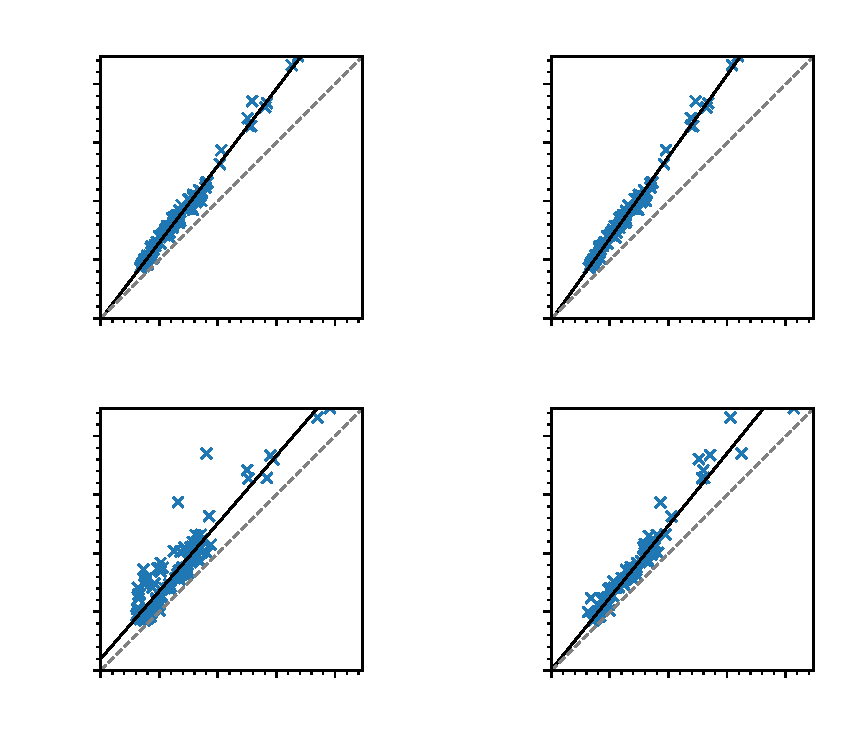
\includegraphics[scale=1.10]{figures/severson_knee_eol_all_algorithms}
%   \caption{Linear regression of knee-point to EOL point}
  \label{fig:kneepoint2EOL}
% \end{subfigure}%
\caption{Linear relations between identified knees and EOL per knee identification algorithm over the Severson et al. \cite{severson_data-driven_2019} dataset. (a) Bacon-Watts\cite{fermin-cueto_identification_2020}, (b) Kneedle\cite{satopaa_finding_2011}, (c) Tangent-ratio\cite{diao_algorithm_2019} (d) Bisector \gbox{{\tt Greenbank and Howey(cite eventually)}}
}
\label{fig:severson_knee_eol_all_algorithms}
\end{figure}












%%%%%%%%%%%%%%%%%%%%%%%%%%%%%%%%%%%%%%%%%
%%%%%%%%%%%%%%%%%%%%%%%%%%%%%%%%%%%%%%%%%%%%%%%%%

\section{Section 2. Impact of time on knee onset}

Capacity fade plots are typically presented with a cycle-based axis, however, this may obscure the influence of calendar aging phenomena. The influence of time is most notable for the study of variables like charge/discharge rate and rest time, so the results in Figure \ref{fig:discharge-rest_cycle} are replotted with a time-based axis in Figure \ref{fig:discharge-rest_time}. Raw data from the corresponding studies were not available, so the cycle times were estimated from the given C-rates and rest times. The trends in discharge rate and rest time influence on knee onset are largely the same as in the cycle-based figure. However, the change from Figure \ref{fig:discharge-rest_cycle}c to Figure \ref{fig:discharge-rest_time}c suggests that much of the reason that longer rest times at TOC and BOD are bad (at least in this study) is calendar aging, not greater degradation at the voltage extremes.    

\begin{figure}[ht]
\centering
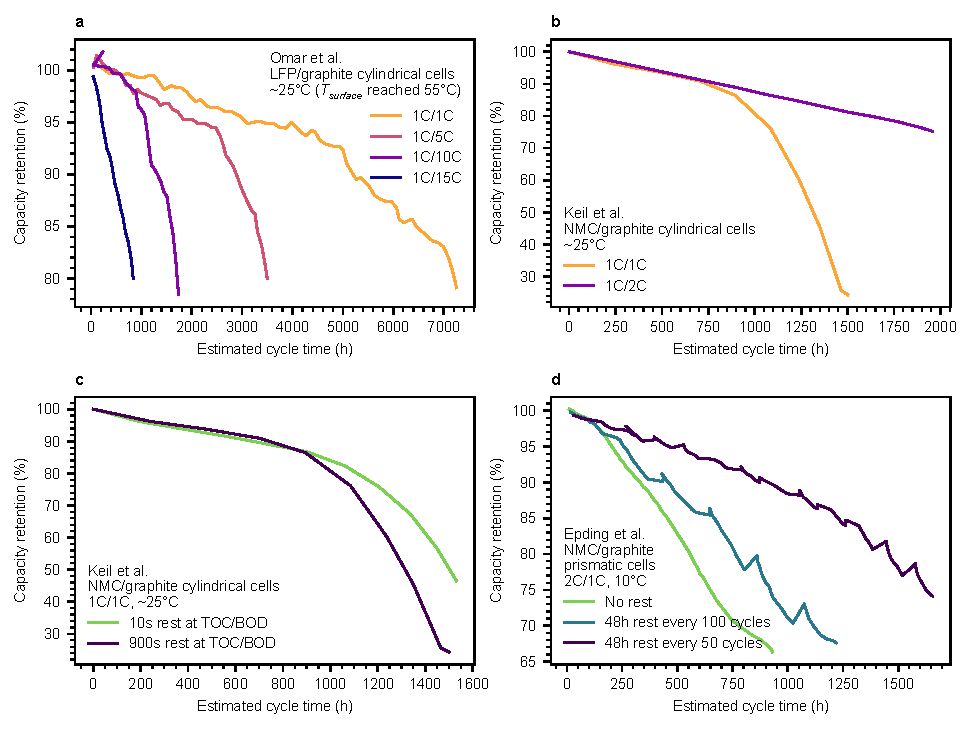
\includegraphics[scale = 1.0]{figures/discharge_rate_rest_time.eps}
\caption{Discharge rate and rest time have mixed effects on knee point onset depending on the testing conditions. Data from Figure \ref{fig:discharge-rest_cycle} replotted with a time-based axis. (a) Higher discharge rate accelerates knee onset. Adapted from Omar et al. \cite{omar_lithium_2014} (b) Lower discharge rate accelerates knee onset. Adapted from Keil et al. \cite{keil_linear_2019} (c) Longer rest time accelerates knee onset. Adapted from Keil et al. \cite{keil_linear_2019} (d) Shorter rest time accelerates knee onset. Adapted from Epding et al. \cite{epding_investigation_2019}.}
\label{fig:discharge-rest_time}
\end{figure}



%%%%%%%%%%%%%%%%%%%%%%%%%%%%%%%%%%%%%%%%%%%%%%
%%%%%%%%%%%%%%%%%%%%%%%%%%%%%%%%%%%%%%%%%%%%%%%%%%%%
%%%%%%%%%%%%%%%%%%%%%%%%%%%%%%%%%%%%%%%%%%%%%%%%%%%%%%%%%
% \bibliographystyle{myIEEEtran}
\bibliography{refs_zotero}

\end{document}